\documentclass[12pt]{article}
% On peut aussi mettre l'option "twoside" [12pt,twoside]

% Packages liées au français
\usepackage[french]{babel}
\usepackage[utf8]{inputenc}
\usepackage[T1]{fontenc}

\usepackage[hyphens]{url}

\addto{\captionsfrench}{%
	\renewcommand{\tablename}{Tableau}
	\renewcommand{\refname}{Bibliographie}
	\renewcommand{\betweenauthors}{&}
}
\renewcommand \figurename{Figure}
\renewcommand \tablename{Tableau} % Nom des tableaux: table -> Tableau
\renewcommand \listfigurename{LISTE DES FIGURES}
\renewcommand \appendixname{ANNEXE}

% Bibliographie
\usepackage{natbib}

% Tableaux et figures
\usepackage{tabu}
\usepackage{array}
\usepackage{graphicx}
\usepackage{amsmath}
\usepackage{amsfonts}
\usepackage{amssymb}
\usepackage{float}
\usepackage{booktabs}
\usepackage{adjustbox}
\usepackage{caption} 
% Multiple figures in a figure
\usepackage{subcaption}

\usepackage{listingsutf8}
\usepackage{listings, lstautogobble}
\usepackage{color}
\definecolor{mygreen}{rgb}{0.1,0.5,0.3}
\lstset{language=TeX,
	basicstyle=\scriptsize,
	commentstyle=\color{mygreen},
	autogobble=true,
	extendedchars=true,
	inputencoding=utf8/latin1,
	rulesepcolor=\color{red}}

% Improve definition
\usepackage{lmodern}
% Spacing
\usepackage{setspace}
% Adjust margins
\usepackage[margin=1.5in]{geometry}

\usepackage{parskip}
\setlength{\parindent}{0pt}

\newcommand{\parder}[2]{\frac{\partial #1}{\partial #2}}

% ------------------------------------------------------------------------ %
% Page Titre
\title{Notions de base pour LaTeX}
\author{Manuel Paquette-Dupuis \\
	et \\
	Stéphane Surprenant}
\date{janvier 2018}
% ------------------------------------------------------------------------ %
\begin{document} 
	% ------------------------------------------------------------------------ %
	\maketitle
	\thispagestyle{empty}
	% ------------------------------------------------------------------------ %
	
	\newpage
	\tableofcontents
	
	\newpage
	\section*{Introduction}
	\doublespacing
	
	LaTeX est un langage qui permet de programmer la mise en forme de textes. Le fait de pouvoir automatiser la mise en forme permet d'assurer une cohérence dans la présentation, en plus de sauver beaucoup de temps en cas d'ajouts, de retraits ou de modification du contenu. Imaginer générer 30 fois un tableau de résultats empiriques et devoir, à chaque fois, l'importer sur un logiciel comme Word et l'ajuster manuellement à chaque fois pour en harmoniser la présentation avec le reste du document. Avec LaTeX, une fois la mise en page programmée, il suffirait simplement de lancer le code après avoir écrasé l'ancien tableau en sauvegardant la nouvelle version. \\ 
	
	Ce document a pour but de vous procurer le strict minimum pour pouvoir apprendre à vous servir de LaTeX. Il y a beaucoup de détails pour lesquels votre meilleur ami sera Google. Pour la rédaction d'une thèse ou d'un mémoire, il serait incroyablement ridicule de ne pas s'en servir, d'autant que les normes de l'ESG sont déjà programmées pour le corps du document, comme pour la bibliographie et que les logiciels statistiques comme EViews, Stata, Matlab, R ou encore SAS ont tous des fonctions permettant d'exporter des figures et des tableaux directement utilisables par LaTeX. Aussi, pour ceux et celles qui n'ont pas encore terminé le cours ECO5072 (Activité de synthèse), vous allez rapidement récupérer l'investissement initial d'apprendre LaTeX en rédigeant les deux rapports exigés. \\
	
	Le document est divisé comme suit: la première partie couvre brièvement l'installation, la seconde partie traite de l'en-tête des documents \url{.tex}, la troisième partie passe en revue un ensemble de fonctions et notions très utilisées et la quatrième partie explique comment utiliser \textit{natbib} conjointement avec le style \textit{apalike-uqam} pour automatiser vos besoins bibliographiques.
	
	\section{Installer LaTeX}
	
	Il vous faut deux logiciels pour utiliser LaTeX: (1) un logiciel pour interpréter le langage et, (2), une interface de travail pour coder et lancer les codes.
	
	\subsection{MikTeX}
	
	Un logiciel permettant à l'ordinateur de <<lire>> le code LaTeX. Voici le lien pour le téléchargement:
	\url{https://miktex.org/download}. Il vous suffit de suivre les instructions pour installer ce logiciel sur votre ordinateur.
	
	\subsection{Interface de programmation}
	
	Ici, il y a plusieurs options. Personnellement, nous utilisons \textbf{TexStudio}: \url{https://www.texstudio.org/}. Certaines de mes collègues utilisent plutôt \textit{TexMaker}: \url{http://www.xm1math.net/texmaker/index_fr.html}. Il suffit d'en choisir un et de l'installer en suivant les instructions.
	
	\subsection{TexStudio}
	
	Une fois que vous avez tout installé, vous pouvez ouvrir votre logiciel de programmation LaTeX. Si vous ouvrez TexStudio, vous allez avoir quelque chose comme ceci: \\
	
	\begin{figure}[H]
		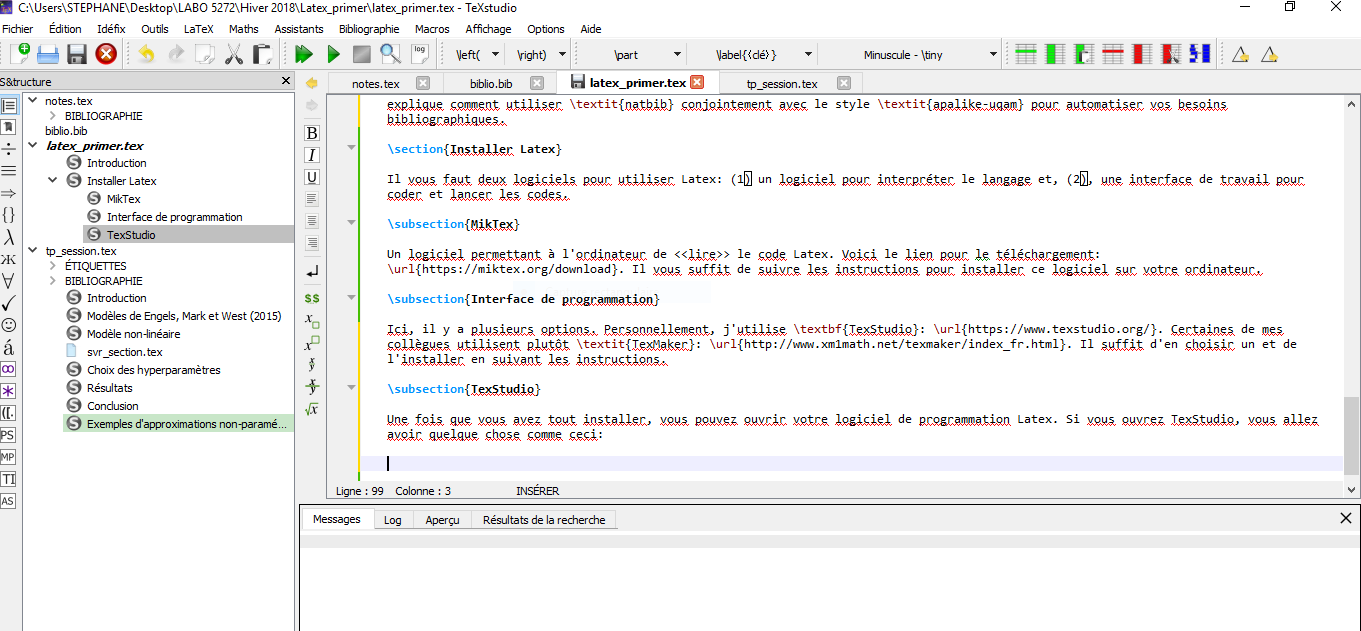
\includegraphics[width=5.5in]{texstudio_screenshot.png}
		\caption{Capture d'écran de TexStudio}
	\end{figure}
	
	À gauche se trouve les documents \url{.tex} ouverts dans TexStudio. Les sections et les documents importés sont aussi visibles pour chaque fichier \url{.tex} utilisé. À droite se trouve le script, c'est-à-dire l'endroit où les commandes sont entrées. La double flèche verte en haut permet d'exécuter le code et de visualiser le document. En bas se trouve une console où des messages, dont des erreurs, s'affichent.
	
	\newpage
	\section{En-tête d'un document LaTeX}
	
	L'en-tête d'un fichier LaTeX commence toujours par la commande \\
	\lstinline|\documentclass[options]{type_de_document}|. Pour un mémoire ou une thèse à l'UQAM, il existe des styles de documents programmés pour une mise en page conforme aux normes de l'université. Pour des travaux, il vous suffit toutefois d'utiliser un style simple comme \textit{article} et d'ajuster les marges. \\
	
	L'en-tête contient aussi d'autres éléments essentiels. D'abord, il faut importer les \textit{packages} utilisés, un peu comme dans R. Voici quelques \textit{packages} utiles:
	
	\begin{lstlisting}[frame=single]
	\usepackage[french]{babel}
	\usepackage[utf8]{inputenc}
	\usepackage[T1]{fontenc}
	\usepackage[hyphens]{url}
	% French
	
	\usepackage{natbib}
	% Bibliography
	
	\usepackage[hyphens]{url}
	% Allowing URLs to be divided between lines
	
	\usepackage{tabu}
	\usepackage{array}     % Matrices (entre autres)
	\usepackage{graphicx}
	
	\usepackage{amsmath}   % Symboles
	\usepackage{amsfonts}
	\usepackage{amssymb}
	
	\usepackage{float}
	\usepackage{booktabs}
	\usepackage{adjustbox} % Compresser un tableau
	\usepackage{caption}   % Titres pour figures et tableaux
	% Tables and figures
	
	\usepackage[margin=1.5in]{geometry} % Marges
	
	\usepackage{setspace} % Fonction double et simple interligne
	\end{lstlisting}
	
	En plus des \textit{packages}, l'en-tête contient aussi des définitions de fonctions. Il vous est possible de modifier des fonctions existantes avec \lstinline|\renewcommand|. Par exemple, \lstinline|\renewcommand{\tablename}{Tableau}| change le nom des titres plaqués par \lstinline|\caption| aux tableaux de l'anglais \textit{table} au français, tableau. \\
	
	Il est aussi possible de créer de nouvelles fonctions avec \lstinline|\newcommand|. Par exemple, vous pouvez créer une fonction pour construire facilement des dérivées partielles comme ceci: \\
	
	\begin{lstlisting}[frame=single]
	\newcommand{\parder}[2]{\frac{\partial #1}{\partial #2}}
	\end{lstlisting}
	
	Si ceci est ajouté à l'en-tête (en plus des \textit{packages mathématiques adéquats}), taper \lstinline|\parder{x}{y}| dans un environnement approprié dans le corps du document renvoit $\parder{x}{y}$. Si vous avez beaucoup de dérivées à taper, ceci allège considérablement le code et sauve un peu de temps. \\
	
	Une dernière chose souvent présente dans l'en-tête est de l'information pour une page de présentation. Par exemple,
	\begin{lstlisting}[frame=single]
	\title{titre}
	\author{nom}
	\date{date}
	\end{lstlisting}
	
	Fait en sorte que la fonction \lstinline|\maketitle| appelée dans le corps du texte produit la page titre que vous voyez au début de ce texte.
	
	\section{Corps}
	
	Le corps d'un document LaTeX est en fait un type d'environnement. Tout environnement dans LaTeX débute par la mention \lstinline|\begin{}| et se termine par \lstinline|\end{}|. Ici, l'environnement est \lstinline|document|.
	
	\subsection{Quelques commandes utiles}
	
	\textbf{Segmenter le texte} \\
	Les commandes \lstinline|\chapter{titre}, \section{titre}, \subsection{titre}| permettent de segmenter le texte tout en conservant une trace des titres, de la hiérarchie des titres et de leur ordre. Cet ordre est reprit lorsqu'on désire insérer une table des matières. La commande \lstinline|\appendix| affecte la numérotation des titres: après cette commande, les titres sont numérotés par des lettres. \\
	
	\textbf{Sauts et ajustements manuels de l'espacement} \\
	\lstinline|\\| indique un saut de ligne, \lstinline|\hspace{}| et \lstinline|\vspace{}| permet d'ajouter des espacements verticaux ou horizontaux -- ou d'enlever de l'espace, si une mesure négative est utilisée. De même \lstinline|\\[ ]| permet un saut de ligne et d'enlever de l'espace si la valeur indiquée entre crochet (par exemple, \lstinline|\\[-5ex]|) est négative. \\
	
	\textbf{Commandes particulières} \\
	<< \lstinline|\| >> permet souvent d'utiliser des caractères fonctionnels de façon textuelle. Par exemple, \{\} encadre souvent des arguments pour des commandes LaTeX. Pour se servir de \{ textuellement, il faut ajouter << \lstinline|\| >>. De même, \% indique le début d'un commentaire. Si on désire l'utiliser textuellement, il suffit d'ajouter << \lstinline|\| >> devant. \\
	
	Exemples: \lstinline|\{\}, \[\], \% |.
	
	Des commandes comme \lstinline|$.$| et \lstinline|\[  \]| permettent d'écrire sur une ligne de texte des expressions habituellement utilisées dans des environnements mathématiques. Par exemple,
	
	\begin{lstlisting}[frame=single]
	\begin{equation}
	y_t = X_t \beta + \epsilon_t
	\end{equation}
	
	$y_t = X_t \beta + \epsilon_t$
	\end{lstlisting}
	
	Sont deux façons de produire une équation. Toutefois, la première crée l'équation dans l'environnement \textit{equation}. Par défaut, ceci la met à part et ajoute une numérotation et, la seconde, inscrit l'équation directement dans une ligne de texte:
	
	\begin{figure}[H]
		\begin{equation}
		y_t = X_t \beta + \epsilon_t
		\end{equation}
		La seconde version permet d'inscrire $y_t = X_t \beta + \epsilon_t$ au beau milieu d'une phrase.
		\caption{Deux façons d'écrire des équations}
	\end{figure}
	
	Il existe typiquement des commandes pour écrire dans le texte des expressions qui seraient normalement illisibles pour LaTeX. Chercher les commandes dites \textit{in line} correspondant à l'environnement de votre choix.
	
	\subsection{Environnements importants}
	
	\textbf{\textit{Figures}} \\
	Dans LaTeX, certaines commandes ne sont lisibles que dans certains environnements. Par exemple, les expressions pour créer des indices, des fractions ou des lettres grecques sont lisibles dans les environnements \textit{equation} ou encore \textit{align}, mais pas dans l'environnement \textit{document} directement. Certains environnements permettent plusieurs lignes (par exemple, \textit{align}), alors que d'autres non (par exemple, \textit{equation}). Vérifiez que les expressions que vous utilisez sont cohérentes avec l'environnement dans lequel elles se 
	trouvent si jamais des erreurs surviennent. \\
	
	\textbf{Un exemple d'environnement \textit{figure}} \\
	\begin{lstlisting}[frame=single]
	\begin{figure}[H]
	\begin{subfigure}{.5\textwidth}
	\includegraphics[width=2.3in]{../50_figures/f_13.png} 
	\end{subfigure}%
	\begin{subfigure}{.5\textwidth}
	\includegraphics[width=2.3in]{../50_figures/f_14.png}
	\end{subfigure}
	\begin{subfigure}{.5\textwidth}
	\includegraphics[width=2.3in]{../50_figures/f_15.png}
	\end{subfigure}%
	\begin{subfigure}{.5\textwidth}
	\includegraphics[width=2.3in]{../50_figures/f_16.png}
	\end{subfigure}
	\begin{subfigure}{.5\textwidth}
	\includegraphics[width=2.3in]{../50_figures/f_17.png}
	\end{subfigure}\\[-1em]
	\caption{Titre de la figure}
	\begin{footnotesize}
	Note: Quelques notes sous la figures.
	\end{footnotesize}
	\end{figure}
	\end{lstlisting}
	
	L'environnement \textit{subfigure} permet de combiner plusieurs figures dans une seule. \lstinline|[width=2.3in]| est une option permettant de fixer les dimensions des petites sous-figures. \lstinline|\caption| définie un titre, \lstinline|\includegraphics| importe un fichier en tant qu'image. LaTeX cherche par défaut dans le répertoire dans lequel se trouve le document \url{.tex} qui est exécuté. Si vous travaillez à partir d'un fichier de travail dans lequel se trouve un répertoire << 30\_latex >> et un répertoire << 50\_figures >>, respectivement pour le document \url{.tex} et les figures, il est utile d'utiliser ce qui s'appelle des \textbf{chemins relatifs}.\\
	
	Pour revenir en arrière d'un dossier, deux points (..) sont entrés avant la première séparation. Dans notre cas, si le dossier << Travail >> contient les deux dossiers susmentionnés, \lstinline|{../50_figures/f_16.png}| indique qu'il y a un répertoire nommé << 50\_figures >> dans << Travail >> (soit un niveau au-dessus de << 30\_latex >>) et que le fichier \url{f_16.png} s'y trouve. Notez que dans LaTeX, les chemins sont indiqués par des \textit{forward slash} et non des \textit{backslash}. Notez que l'importation ne se limite pas aux figures. Vous pouvez importer des fichiers \url{.tex} avec la commande \lstinline|\input{}|. Les tableaux extraits de logiciels statiques sont souvent sauvegardés en format \url{.tex} pour permettre leur importation de cette façon. \\
	
	L'environnement \textit{footnotesize} réduit la taille du texte. Les \% indique comment organiser les sous-figures (soit une à côté de l'autre plutôt qu'une au-dessus de l'autre). \\
	
	\textbf{Exemple de l'environnement \textit{Table}} \\
	
	\begin{lstlisting}
	\begin{table}[H]
	\begin{center}
	\caption{Tests de saisonnalit\'{e} Kruskal-Wallis} \label{kw_test}  \small\small                                                                                                                                                                                                    
	\begin{tabular}{lcccccc} \toprule\toprule                                                                                                                                                                                                                                           
	& \multicolumn{3}{c}{$\Delta ln A_t^{(2)}$} &\multicolumn{3}{c}{$\Delta ln Y_t$} \\                                                                                                                                                                                                 
	&  KW  &  DL  &  Valeur p  &  KW  &  DL  &  Valeur p  \\ \midrule                                                                                                                                                                                                                   
	Canada (T)  & 3,0494  & 11  & 0,9901  & 431,7969  & 11  & 0  \\                                                                                                                                                                                                                     
	Canada (B)  & 4,9891  & 11  & 0,9317  & 451,9053  & 11  & 0  \\                                                                                                                                                                                                                     
	Canada (S)  & 1,6952  & 11  & 0,9993  & 384,0472  & 11  & 0  \\                                                                                                                                                                                                                     
	Terre-Neuve (T)  & 3,1991  & 11  & 0,9878  & 405,7299  & 11  & 0  \\                                                                                                                                                                                                                
	Terre-Neuve (B)  & 9,6117  & 11  & 0,5656  & 379,6131  & 11  & 0  \\                                                                                                                                                                                                                
	Terre-Neuve (S)  & 1,5735  & 11  & 0,9995  & 352,1401  & 11  & 0 
	\\  \bottomrule\bottomrule                                                                                                                                                                               
	\end{tabular}    
	\end{center}     
	\begin{footnotesize}  
	\flushleft     
	Notes: 
	\end{footnotesize}   
	\end{table}  
	\normalsize
	\end{lstlisting}
	
	L'environnement \textit{center} centre le texte, la commande \lstinline|\multicolumn{a}{b}{c}| permet à l'expression \textit{c} de couvrir \textit{a} colonnes de façon \textit{b}. Les justifications pour \textit{b} sont centrée (c), à gaucher (l) et à droite (r). Le même principe s'applique à l'argument de l'environnement \textit{tabular}. Les expression \& séparent les colonnes et \lstinline|\\| séprarent les lignes dans l'environnement \textit{tabular}. Les commandes \lstinline|\bottomrule, \toprule, \midrule| crées des traits horizontaux. \lstinline|\small| et \lstinline|\normalsize| ajuste la taille du texte. Les expressions comme \lstinline|\'{e}| sont des commandes natives de LaTeX pour créer des accents -- dans ce cas-ci, le résultats est <<é>>. Ce n'est pas nécessaire si nous avons les bons \textit{packages}. \\
	
	Finalement, l'ajout de \lstinline|\label{kw_test}| permet de créer un objet de référence. Avec ceci, à tout endroit dans le texte où se trouve \lstinline|\ref{kw_test}|, le numéro du tableau sera reproduit. De cette façon, si on décide de changer l'ordre des tableaux, le texte s'ajuste en conséquence et nous n'avons pas à chercher des chiffres entrés manuellement pour les changer. Cette commande fonctionne aussi pour les figures, les sections, les sous-sections, les chapitres et les équations.\\
	
	\textbf{\textit{Align et equation}} \\ 
	
	L'environnement \textit{align} nécessite le package \textit{asmath}. Il fait partie des environnements les plus simples pour écrire une série d'équations ou faire une démonstration.
	
	\textbf{Exemple de l'environnement \textit{align}} \\
	\begin{lstlisting}[frame=single]
	\begin{align*}
	\hat{\beta} &= arg \min_{\beta}\{u'u\} \\
	&= arg \min_{\beta}\{(Y - X\beta)'(Y - X\beta)\} \\
	&= arg \min_{\beta}\{Y'Y - Y'X\beta - \beta'X'Y - \beta'X'X\beta\} \\
	&= arg \min_{\beta}\{Y'Y - 2Y'X\beta - \beta'X'X\beta\} \\
	\end{align*}
	\end{lstlisting}
	
	Cette exemple présente le problème de minimisation des moindres carrés ordinaires. L'étoile (\url{*}) après align indique que les équations ne seront pas référencées. Si ce symbole est omis, les équations seront associées à des nombres et pourront être référencées dans le texte. Les symboles mathématiques, les lettres grecques et le texte peuvent être insérés librement dans cet environnement. L'ajout du symbole esperluette (\url{&}) alignera les équation verticalement. Ce code produit :
	\begin{align*}
	\hat{\beta} &= arg \min_{\beta}\{u'u\} \\
	&= arg \min_{\beta}\{(Y - X\beta)'(Y - X\beta)\} \\
	&= arg \min_{\beta}\{Y'Y - Y'X\beta - \beta'X'Y - \beta'X'X\beta\} \\
	&= arg \min_{\beta}\{Y'Y - 2Y'X\beta - \beta'X'X\beta\} \\
	\end{align*}
	
	\textbf{Exemple de l'environnement \textit{equation}} \\
	
	\begin{lstlisting}[frame=single]
	\begin{equation}
	\hat{\beta} = (X'X)^{-1}X'Y
	\label{MCOeq}
	\end{equation}
	\end{lstlisting}
	
	Pour afficher une équation unique, il est préférable d'utiliser l'environnement \textit{equation}. Cet exemple permet d'afficher l'estimateur des moindres carrés ordinaires. Il sera possible de faire référence à cette équation dans le texte, comme pour les tableaux, à l'aide de \lstinline|\ref{MCOeq}|.
	
	\begin{equation}
	\hat{\beta} = (X'X)^{-1}X'Y
	\label{MCOeq}
	\end{equation}
	
	\section{Bibliographie}
	
	L'utilisation de LaTeX permet de faciliter grandement la présentation d'une bibliographie. La majorité des moteurs de recherches d'articles scientifiques (Google Scholar, IDEAS, NBER, etc.) offre la possibilité d'exporter les références en format BibTeX, le format utilisé par LaTeX pour créer des bibliographies. Pour introduire une bibliographie dans un document il faut d'abord créer un fichier \url{.bib} qui contiendra chacune des références. Pour ce faire, à partir de l'interface de programmation, créer un nouveau fichier (raccourci clavier ctrl+n) et l'enregistrer avec l'extension \url{.bib}. Par exemple, \url{bibliographie_TP1.bib} pourrait être utilisé.
	
	Ensuite, il faut lier le fichier créé au texte auquel une bibliographie doit être ajoutée. 
	\begin{lstlisting}[frame=single]
	\clearpage
	\bibliographystyle{apalike-uqam.bst}
	\bibliography{bibliographie_TP1.bib}
	\end{lstlisting}
	
	Ici, la commande \lstinline|\clearpage| permet d'afficher la bibliographie à la fin du texte. Ensuite, \lstinline|\bibliographystyle{num_du_style.bst}| permet de sélectionner le style d'affichage des références dans la bibliographie. Pour le style de l'UQAM, il suffit d'utiliser le fichier \url{apalike-uqam.bst} en l'incluant dans l'espace de travail. Finalement, la commande \lstinline|\bibliographie{nom_du_fichier.bib}| affiche la bibliographie.
	
	Pour citer facilement des articles à partir d'un moteur de recherche, il faut trouver la référence BibTeX associée à l'article. Par exemple, pour Google Scholar l'option se trouve sous le sommaire. 
	
	\begin{figure}[H]
		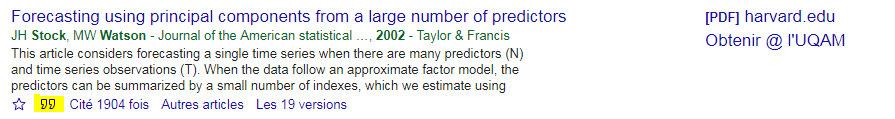
\includegraphics[width=5.5in]{googleScholar.png}
		\caption{Exemple pour un article de Stock et Watson sur Google Scholar}
	\end{figure}
	
	Par la suite, sélectionner l'option BibTeX. Elle est surlignée en jaune dans la figure \ref{optionbib}.
	\begin{figure}[H]
		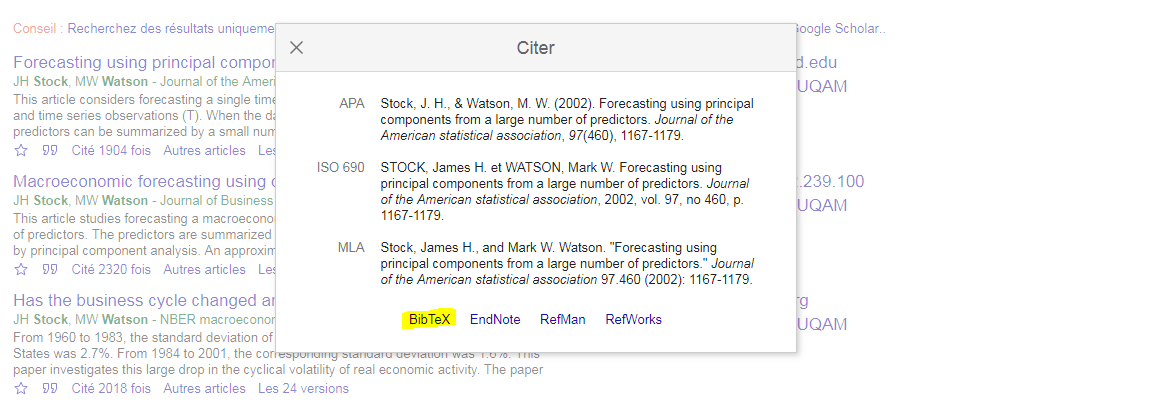
\includegraphics[width=5.5in]{googleScholar2.png}
		\caption{Option BibTeX sur Google Scholar}
		\label{optionbib}
	\end{figure}
	
	Le résultat s'affichera sur une page web vierge.
	
	\begin{figure}[H]
		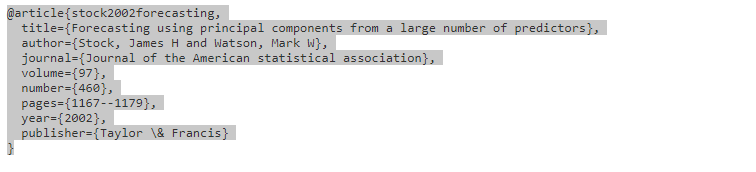
\includegraphics[width=5.5in]{googleScholar3.png}
		\caption{Référence BibTeX provenant de Google Scholar}
		\label{gscholar}
	\end{figure}
	
	Pour finir, copier la référence dans le document \url{.bib} créé plus tôt. Les autres références seront dans le même fichier, pour créer une liste de tous les références à citer.
	
	\begin{figure}[H]
		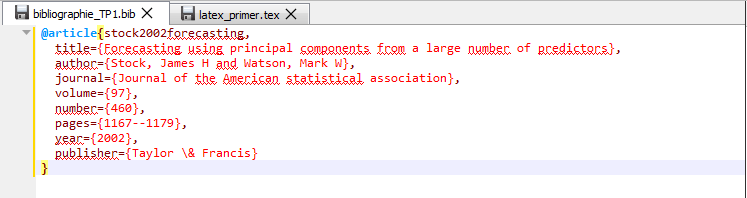
\includegraphics[width=5.5in]{googleScholar4.png}
		\caption{Référence BibTeX copiée dans le document .bib}
	\end{figure}
	
	Maintenant, dans le texte il est possible de citer les articles en utilisant le code associé à la référence BibTeX. Pour l'exemple de l'article de Stock et Watson, ce code est donné par \url{stock2002forecasting}. Pour les références dans le texte, sous forme auteur date, il faut utiliser la package natbib (à l'aide de la commande \lstinline|\usepackage{natbib}| dnas l'entête). Ce package permettra notamment les deux types les plus fréquemment utilisés soit avec et sans parenthèses. La commande \lstinline|\citet{stock2002forecasting}| affichera \citet{cit1} alors que \lstinline|\citep{stock2002forecasting}| affichera \citep{cit1}. 
	
	\clearpage
	\bibliographystyle{apalike-uqam.bst}
	\bibliography{bibliographie}
	
\end{document}
